\begin{theo}[Impuls]{Impuls}
    Impuls is een vectoriële grootheid die de hoeveelheid van beweging weergeeft. In formulevorm: 
        \begin{equation*}
            \Vec{p} = m\Vec{v}.
        \end{equation*}
        
    \noindent Met dit nieuw begrip kunnen we de tweede wet van Newton herdefiniëren:
    \begin{equation*}
        \sum \Vec{F} = m\Vec{a} = \dfrac{d(m\Vec{v})}{dt} = \dfrac{d\Vec{p}}{dt}.
    \end{equation*}

    \vspace{-0.3cm}

    % \noindent \textbf{Opmerking:} Om het impuls van een voorwerp te veranderen is een kracht nodig!
\end{theo}

\begin{lem}[Behoud van impuls]{Behoud van impuls}
    De wet van de behoud van impuls stelt dat de \textbf{totale impuls} ($ \Vec{P} $) van een geïsoleerd stelsel van deeltjes constant is wanneer: 
    \begin{equation*}
         \sum \Vec{F}_{ext} = \dfrac{\sum_i d\Vec{p}_i}{dt} = \dfrac{d\Vec{P}}{dt} = 0.
    \end{equation*} 
    % \noindent \textbf{Dus:} De verandering van impuls is gelijk aan de \textbf{netto}kracht op het systeem.
\end{lem}

\begin{app}[Elastische botsing]{Elastische botsing}

    Bij een elastische botsing wordt de kinetische energie behouden. We kunnen nu met deze wet en de wet van behoud van impuls te werk gaan. Enerzijds krijgen we uit de wet van behoud van impuls: 
    
    \begin{equation}
        m_av_a + m_bv_b = m_av_a' + m_bv_b'
    \end{equation}
    
    \noindent Anderzijds uit de wet van behoud van kinetische energie bij elastische botsing:
    \begin{equation}
        \dfrac{1}{2}m_av_a^2 + \dfrac{1}{2}m_bv_b^2 = \dfrac{1}{2}m_a{v_a'}^{2} + \dfrac{1}{2}m_b{v_b'}^{2}
    \end{equation}
    
    \noindent We kunnen (1) herschrijven als volgt:
    
    \begin{equation}
        m_a(v_a - v_a') = m_b(v_b' - v_b)
    \end{equation}
    
    \noindent We kunnen ook (2) herschrijven als volgt:
    
    \begin{equation}
        m_a(v_a^2 - {v_a'}^{2}) = m_b({v_b'}^{2} - v_b^2)
    \end{equation}
    
    \noindent Wegens $ (a-b)(a+b) = a^2-b^2 $ kunnen we (4) weer herschrijven:
    
    \begin{equation}
        m_a(v_a - v_a')(v_a + v_a') = m_b(v_b' - v_b)(v_b' + v_b)
    \end{equation}

    % \newpage
    
    \noindent Tenslotte kunnen we (5) delen door (3) en bekomen we:

    \vspace{-0.3cm}
    
    \begin{align*}
        v_a - v_b  &= -(v_a' - v_b') 
    \end{align*}
    
    % \noindent Dit is een interessant resultaat: het vertelt ons dat bij elke elastische head-on botsing de relatieve snelheid van de twee voorwerpen na de botsing dezelfde grootte (maar tegengestelde richting) heeft als vóór de botsing, ongeacht de massa's. 

    \vspace{-0.3cm}

\end{app}
    
\begin{app}[Inelastische botsing]{Inelastische botsing}
    
    Bij een inelastische botsing wordt de kinetische energie niet behouden. Desondanks wordt de totale energie altijd behouden en dus ook het vectoriële totale impuls. Als de botsing compleet inelastisch is (dus dat de voorwerpen één massa vormen na botsing), dan kunnen we de wet van behoud van impuls toepassen en de volgende formule krijgen:
    
    \begin{equation*}
        m_a\Vec{v}_a + m_b\Vec{v}_b = (m_a + m_b)\Vec{v}'
    \end{equation*}

\end{app}

% \begin{ex}[Voorbeeld: Botsingen in meerdere dimensies]{Botsingen in meerdere dimensies}
%     \centering
%     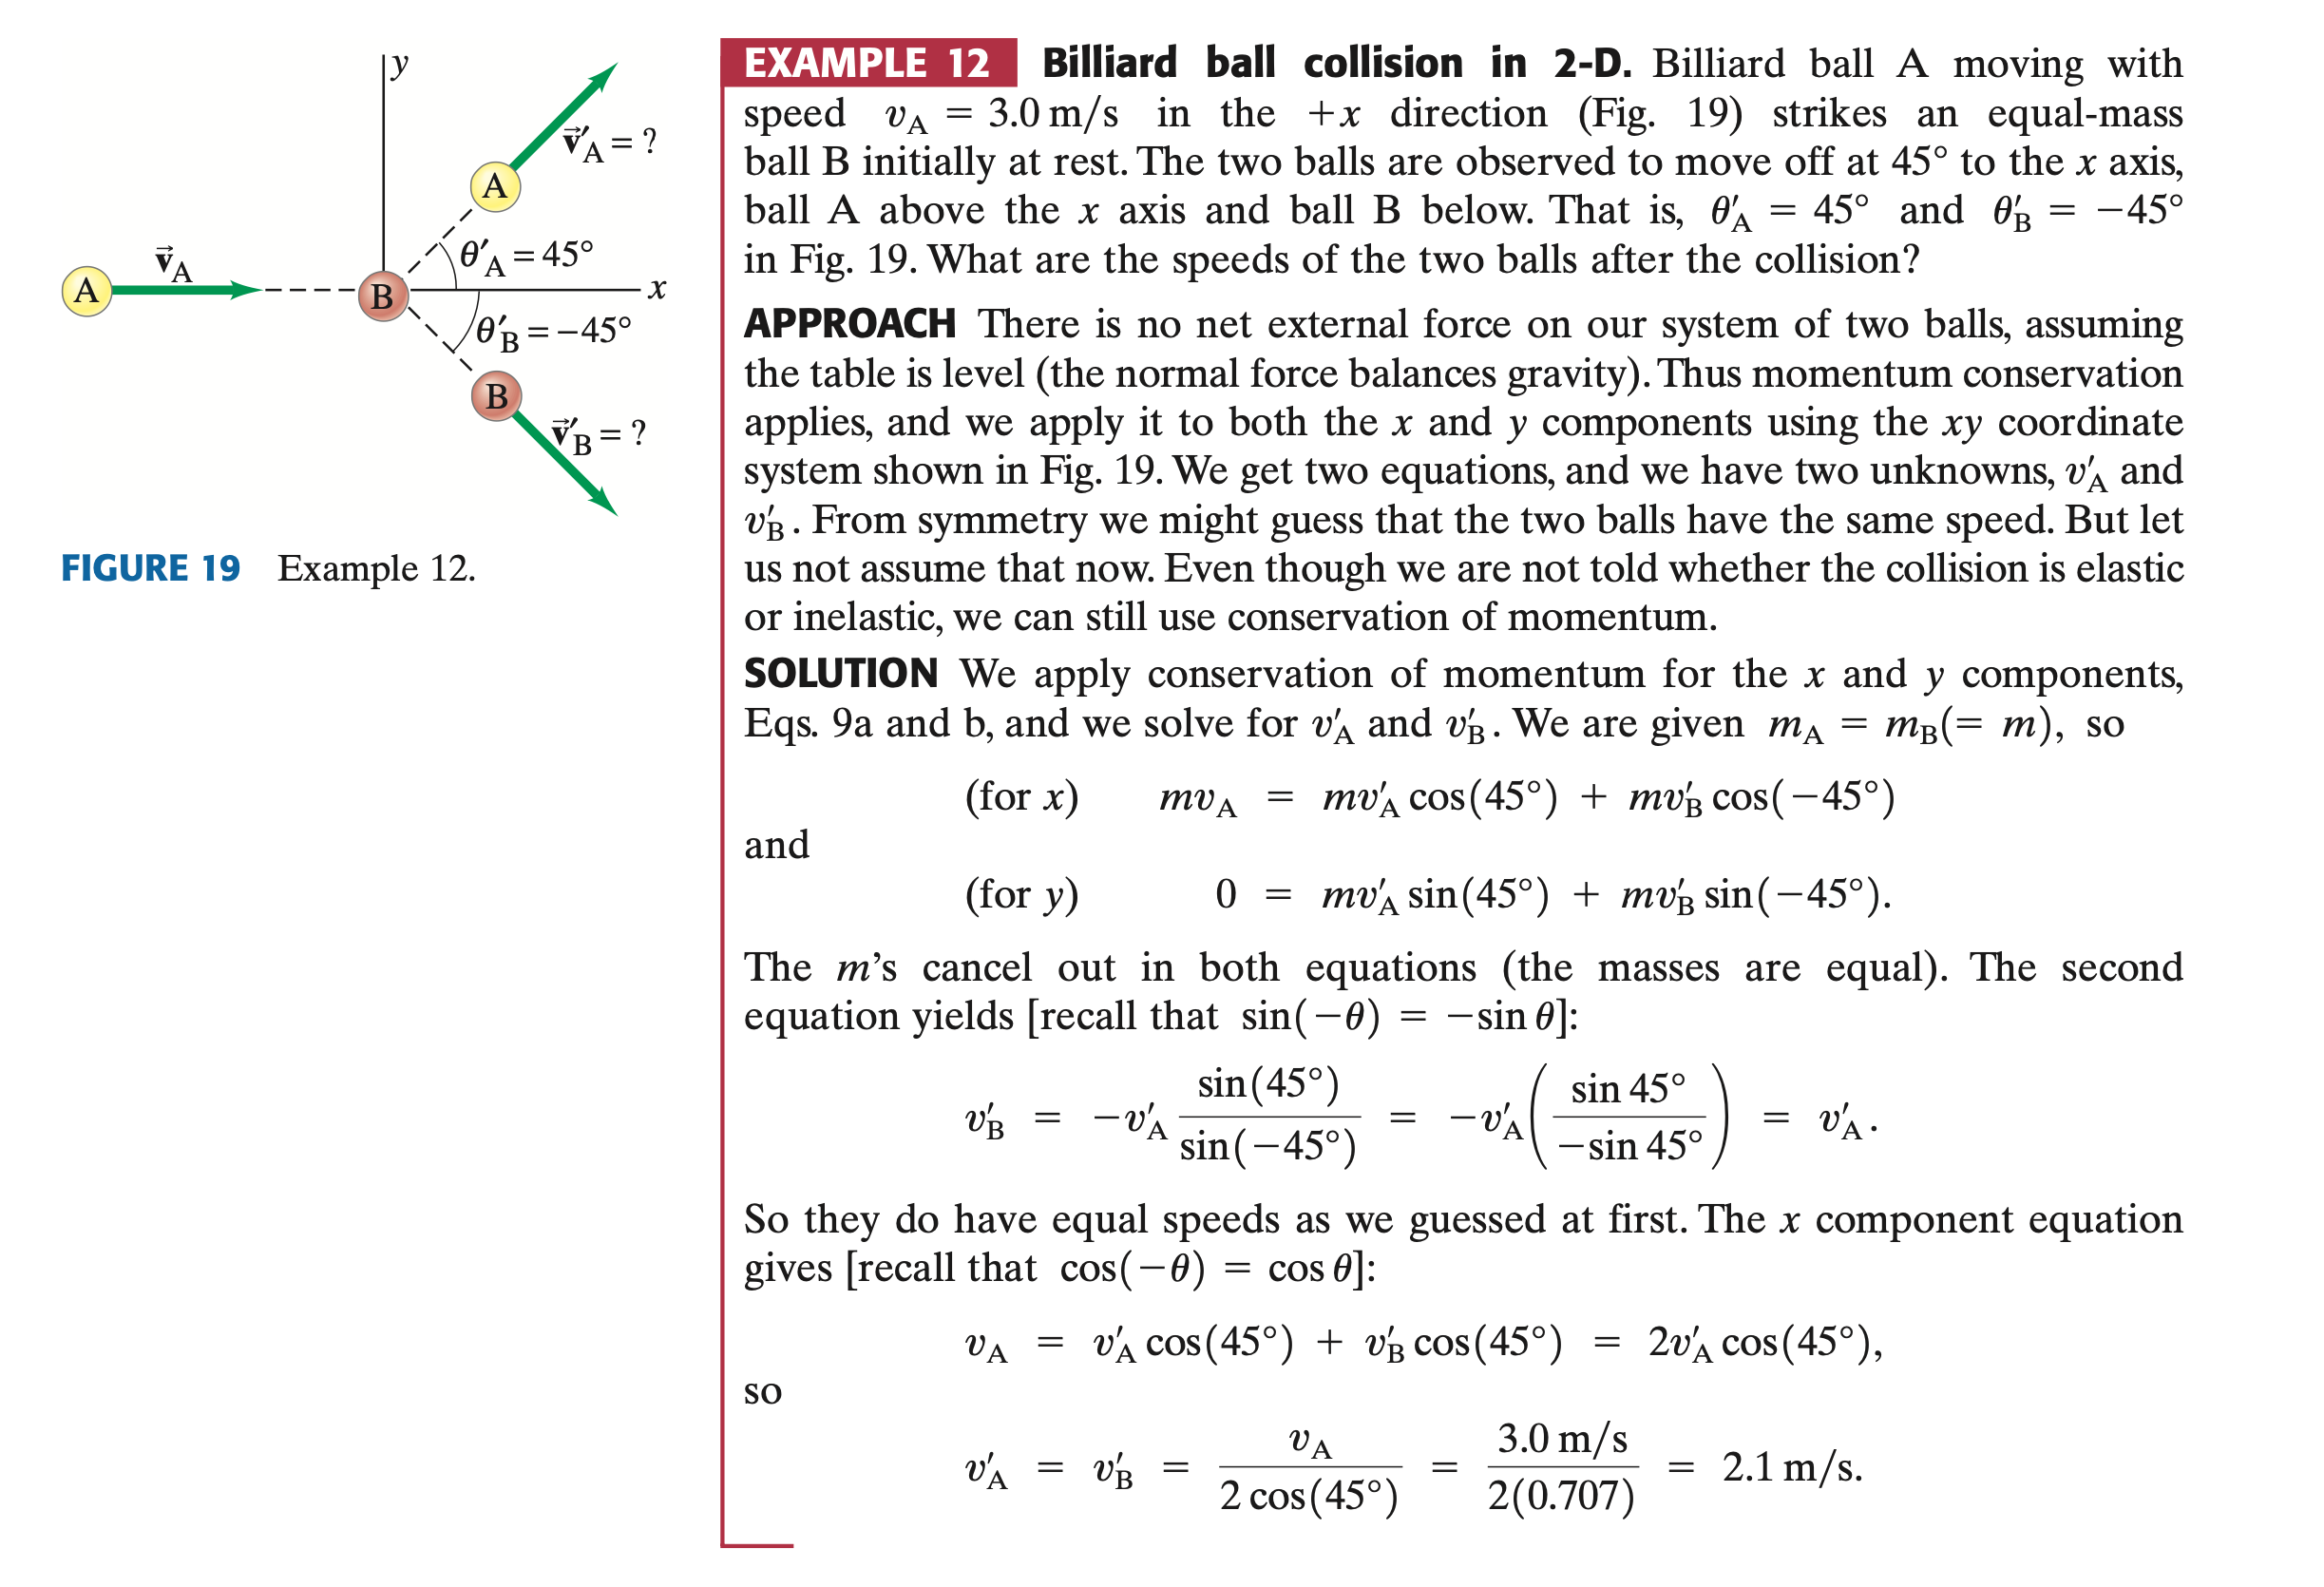
\includegraphics[scale = 0.36]{Examples/Dynamica/9.12.png}
% \end{ex}
